%!TEX root = schedCompPres.tex 

% General Goal: I want you to add this into your scheduling
% strategies.  
% General Goal: Tell audience that what I'm doing is relevant. 
% Specific Goal: Tell audience that low-overhead scheduling can
% benefit the energy efficiency for the product/application that you
% are creating - making money for the company. 

% TODO:L5: Practice presentation. 

% TODO: L4: Write presentation transitions 

% TODO: L4: Decide what to do for the application program timelines.
% -done 

% TODO:L0: add motivation for scheduler composition. - done 

% TODO:L4: Fix slide on schedulers. 

% TODO: L0: add experimental setup =  - done 
% TODO: L0: add descriptions for each scheduler  
%TODO:L3: check numbering and consistency 
%TODO: think about how to present snap 
%TODO: go through transitions and practice in morning 
%TODO: think about title 
%TODO: check that sentence comes at beginning. 
%TODO: add in a proper stencil code
\comments{
\begin{frame} 
\frametitle{Using Threading for PlasComCM}
\begin{center} 
{\tiny Insert 4 OpenMP low-overhead scheduling slides here.}
\end{center} 
\end{frame} 
}

\comments{
  \begin{frame}[label=lastslide]
    \frametitle{Current Work with GPUs}
    \begin{itemize}
      \item Working with scientists in physics and mechanical sciences to integrate my techniques in a real-world CFD application.
      \item Apply work in the context of heterogeneous
        architectures. 
       \item Use loop scheduling ideas on MIC. 
    \end{itemize}
  \end{frame}
}

\begin{frame}[label=synchMPICode]
\frametitle{Sample MPI Code} 
%common pattern 
\visible<1->{\small Common pattern in application codes.\\
% e.g., in~\hyperlink{appCodesAndSetup}{ones}\comments{\hyperlink{}{SNAP}, \hyperlink{}{miniFE}, \hyperlink{}{Rebound},} we'll see later.\comments{, we'll see
%in the experimentation section later.}
}
%\visible<1->{\lstinputlisting{./listings/mpi-bulk-synch.c}}
\visible<1->{\lstinputlisting{./listings/1DstencilUsingMPI.c}}
%\visible<2->{\lstinputlisting{./listings/mpi-synch-code-inst.c}} 
\vspace{0.1in}
\visible<1->{\small Assuming this code is perfectly load balanced,
  should be no performance problems.}
\end{frame}

\comments{
\begin{frame}[label=transImbMitigation]
  \frametitle{Transient Load Imbalance and its Mitigation}
  \begin{columns}
    \column{0.5\columnwidth}
    \visible<1->{\small Infrequent noise $\rightarrow$ slowdown at
      scale.}
    %TODO: slowdown?                                                  
    \column{0.5\columnwidth}
    \visible<1->{{\small \comments{$\exists$ large \# cores / node
          $\rightarrow$}Idea for fix: redistribute within node.}}
  \end{columns}
  %TODO: animate this to show  right one slide later.     
%  \visible<1->{
%    \begin{figure}[ht!]
%      \label{fig:NoiseTransImbPic}
%      \label{fig:AmplificationPic1}\subfloat[\label{fig:AmplificationPic1}
%        \tiny Noise\comments{different nodes in different iterations}
%        delays almost every
%        iteration.]{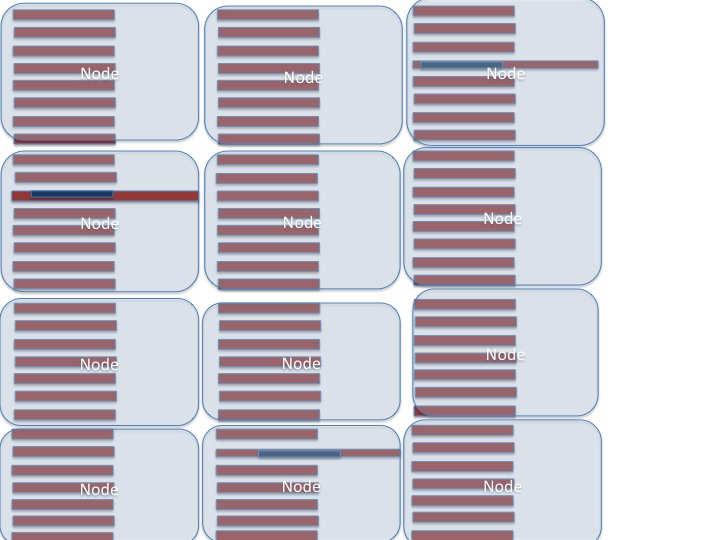
\includegraphics[height=1.3in]{./pictures/Noise}}}\visible<1->{\label{fig:AmplificationPic3}\hspace*{0.25in}\subfloat[\label{fig:AmplificationPic3}{\tiny
%        Performance improves, assuming perfect work re-distribution within each node. } %can be perfectly
      %re-distributed within each node.                        
%  ]{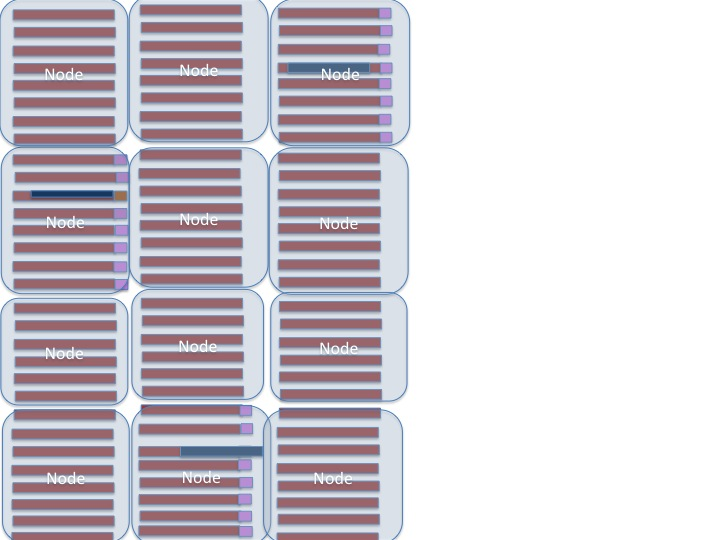
\includegraphics[height=1.3in]{./pictures/NoiseMitigated}}\caption{\label{fig:NoiseTransImbPic}
%      Application timeline schematics.}}
%    \end{figure}
\end{frame}


\begin{frame}[label=mitigationWithinNode]
\frametitle{Within-node Persistent Load Imbalance and Mitigation}
\begin{figure}[ht!]
\label{fig:AppPersistentImbPic}
\subfloat[\tiny Application
  imbalances.]{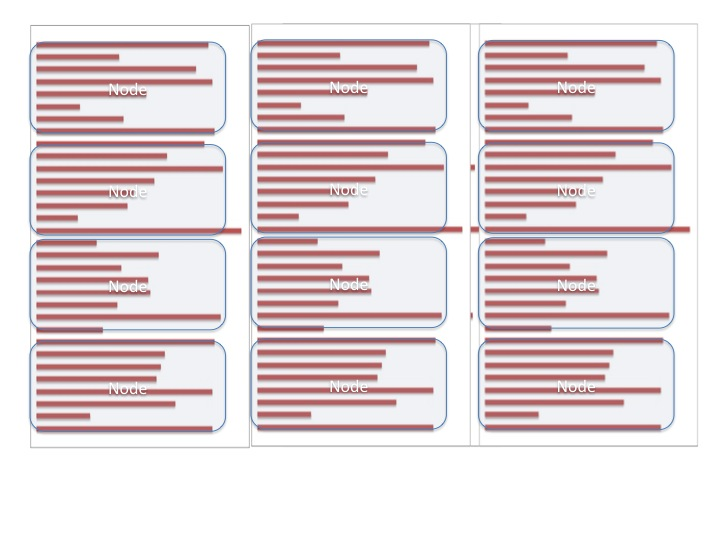
\includegraphics[height=1.3in]{./pictures/PersistentImb2}}\label{fig:AmplificationPic3}\hspace*{0.25in}\subfloat[\label{fig:AmplificationPic3}\tiny
  Mitigated by within-node
  re-distribution.]{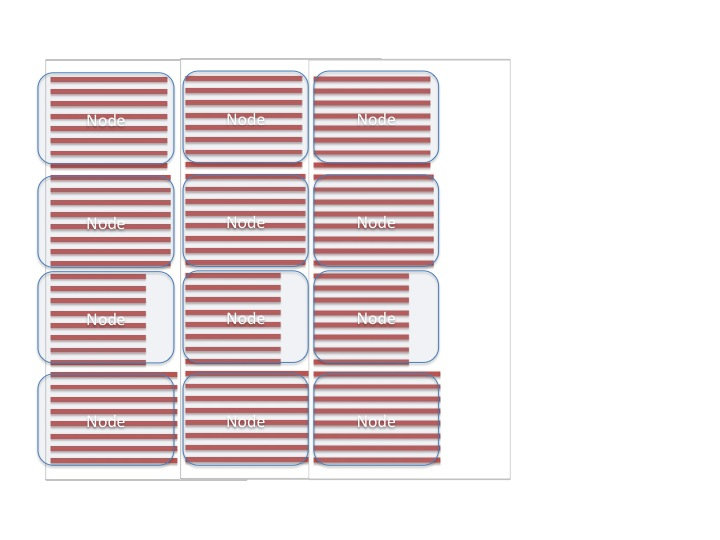
\includegraphics[height=1.3in]{./pictures/PersistentOptimized}}
%\caption{\label{fig:AppPersistentImbPic} Application-induced load
%imbalances.}                                      
\end{figure}
{\small Indent due to not doing across-node balancing, but still much
  better than before.}
\end{frame}

}

%TODO: see if we can change title                           
\comments{ 
\begin{frame}[label=dynLoadBal]
\frametitle{$\rightarrow$ Can Dynamic Load Balancing Fix This?}
\begin{itemize}
\item \small Dynamic load balancing within a node has potential to mitigate imbalances, {\it if} it can be done efficiently.
%\item Dynamic                                              

\begin{itemize}
%\item For both kinds of imbalances.                      
\item \small Persistent imbalance can also be addressed by across-node load balancing (available in Charm++, Zoltan), but it requires more complex machinery (and is complementary anyway).\\
%know questions here 
\end{itemize}
\item \small OpenMP supports dynamic balancing.
\item \small Use OpenMP within-node.
%\begin{itemize}              
%\item \small Is this efficient enough?
%\end{itemize}                                 
\vspace*{.5in}
%\item However, within-node dynamic load balancing faces many                                                     
%challenges.                                        
\end{itemize}
\end{frame}


\begin{frame}[label=hybridstatdyn]
 \frametitle{Hybrid Static/Dynamic Scheduling}
\begin{columns}
  \column{0.5\columnwidth}
  \vspace*{-0.2in}
  \lstinputlisting{./listings/threadedCompRegion-static.c}
  \column{0.5\columnwidth}
%  
\includegraphics[scale=0.15]{./images/legend-dynamic}\\                                                              
  \vspace*{-0.2in}
  \begin{center}
    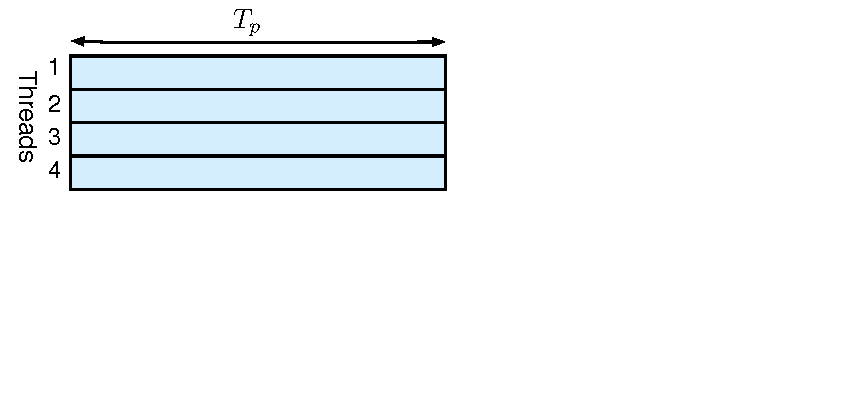
\includegraphics[scale=0.31]{./images/threadedCompRegion-static}
  \end{center}
  \vspace*{-0.4in}
  \begin{center}
    \tiny Susceptible to imbalance.
  \end{center}
\end{columns}
\begin{columns}
\column{0.5\columnwidth}
\vspace*{-0.15in}
\lstinputlisting{./listings/threadedCompRegion-dynamic.c}
\column{0.5\columnwidth}
  \begin{center}
    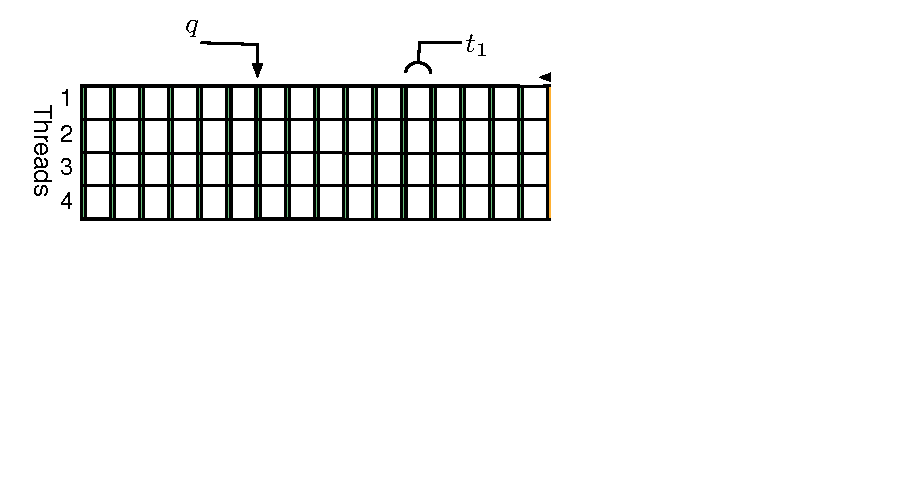
\includegraphics[scale=0.31]{./images/threadedCompRegion-dynamic}
  \end{center}
\vspace*{-0.3in}
\begin{center}
{\tiny Scheduler overhead stretches time.}
\end{center}
\end{columns}
\begin{columns}
\column{0.5\columnwidth}
%TODO: fix code  to be hybrid sched
\vspace*{-0.1in}
\lstinputlisting{./listings/threadedCompRegion-hybrid.c}
\column{0.5\columnwidth}
\begin{center}
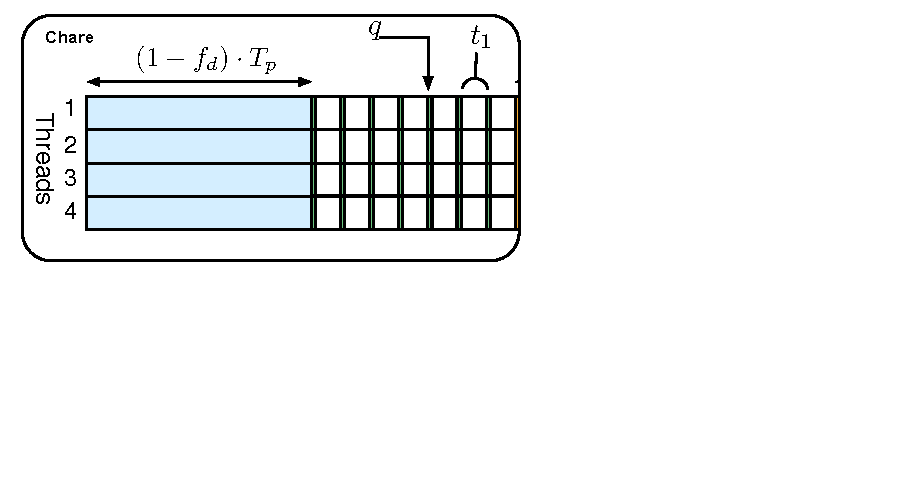
\includegraphics[scale=0.31]{./images/threadedCompRegion-hybrid}
\end{center}
\vspace*{-0.3in}
\begin{center}
{\tiny Can reduce imbalance and sched
  ovhd. simultaneously.\comments{through
    \hyperlink{expTunedSF}{tuning} static fraction.}}
\end{center}
\end{columns}
\end{frame}
}

\begin{frame}[label=halftimings]
\frametitle{Performance with~\hyperlink{expTunedSF}{Tuned} Static Fraction}
\begin{figure}[ht!]
\begin{center}
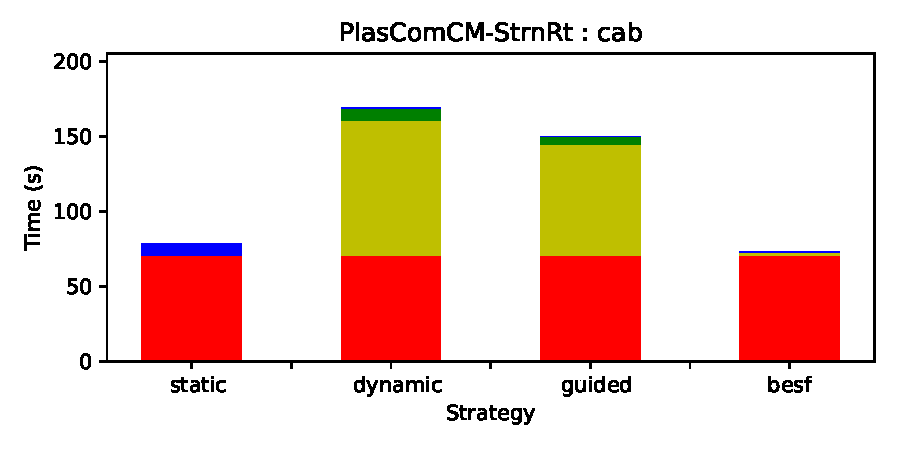
\includegraphics[scale=0.34]{./plots/dmTime-PlasComCM-StrnRt-cab-withbesf}
%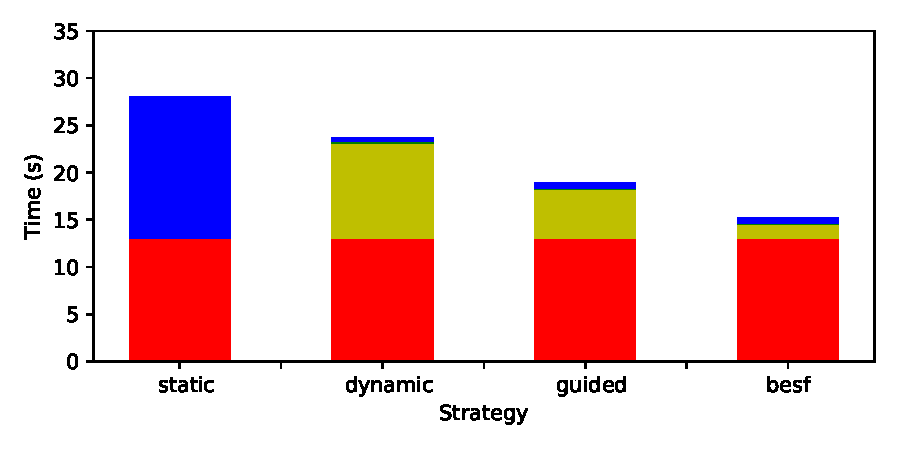
\includegraphics[scale=0.34]{./plots/dmTime-nbody-cab-withbesf}\\
\end{center}
\label{fig:dmTimes-NASLU-cab}
\end{figure}
\begin{center}
{\small In \textit{besf}, we use the best static fraction. See rightmost bar.}
\end{center}
%TODO: fix this so it doesn't duplicate                     
\visible<1->{
\begin{enumerate}
\small \item \small Balances the tradeoff between load balance and
locality
 across applications and platforms. \comments{ Half is better than
   dynamic strategies.  }
\item \small \comments{Even for NASLU,} The \textit{besf} strategy gives performance gains
  over \textit{static}, i.e., the code benefits from the small amount of
  dynamic load balancing.
%\item \tiny Minimizes the costs in each of the three challenges,                                               
%simultaneously.                         
\item \small EuroMPI 2010 : V. Kale and W. Gropp [statdyn] studies
  this idea in more depth.
\end{enumerate}}
\end{frame}

\begin{frame}
\frametitle{PlasComCM Suitability for GPU} 
\begin{itemize} 
\small \item \small PlasComCM has a large number of floating point
operations per grid point per timestep \comments{ $\rightarrow$ easy to vectorize}
\item \small These computations are repeated over
  timesteps \comments{$\rightarrow$ ease of programmability}. 
\end{itemize} 
{\small Can an accelerator architecture provide significant performance
benefit for stencil-type computation on structured grids?} 
\end{frame} 

\begin{frame}[label=perfExp]
\frametitle{Performance Expectation Using GPU} 
\begin{itemize} 
\small \item \small Efficient assuming all data can fit in memory. 
%\item \small How many GPUs needed to fit application data? 
\item \small Consider just the 2D axi-symmetric problem. 
\item \small We only need 1 (allowing data to be held in GPU memory). 
\item \small Future archs may have \texttt{nvlink}, other technology.  
\end{itemize} 
% Be optimistic and theorize. 
\end{frame} 

\comments{
\begin{frame}[label=cid] 
\frametitle{3D 7-point Stencil Results} 
\begin{center} 
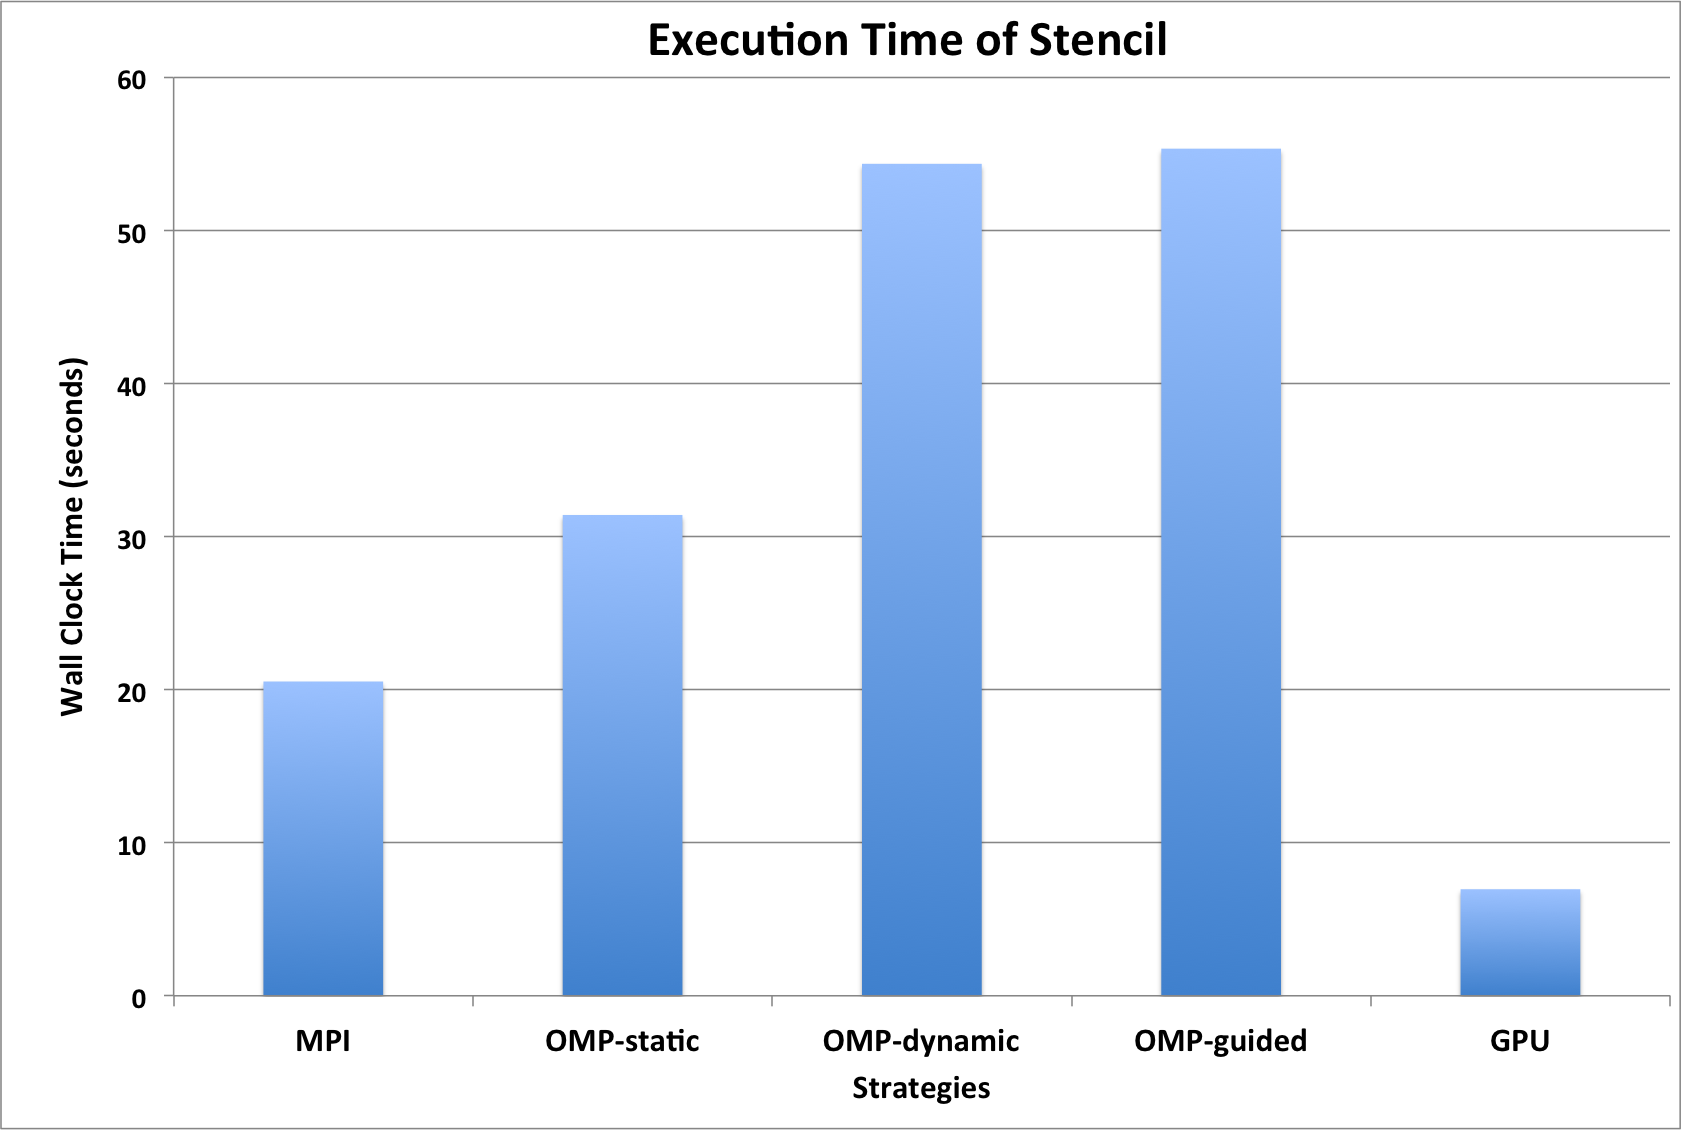
\includegraphics[scale=0.24]{./plots/stencilGPUresults} 
\end{center} 
\end{frame} 


\begin{frame}[label=cid]
\frametitle{PlasComCM Results/Projections for CID} 
\begin{center}
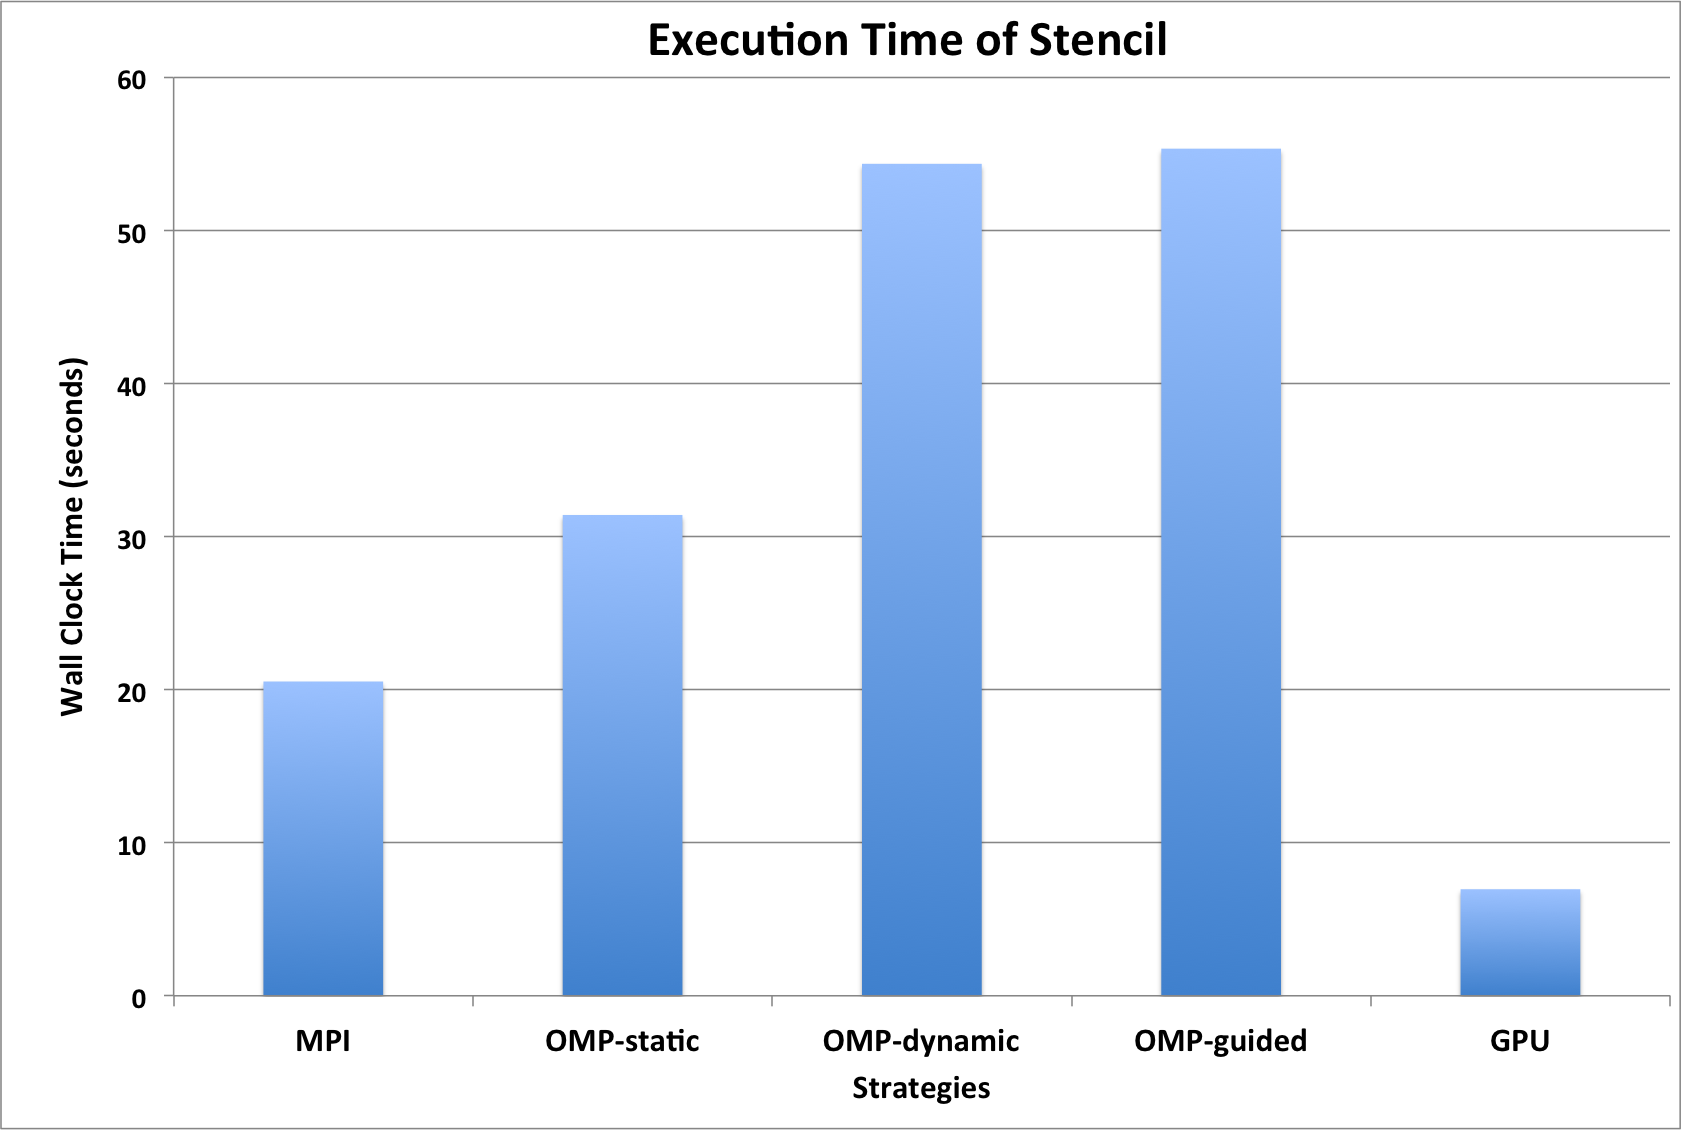
\includegraphics[scale=0.18]{./plots/stencilGPUresults} \hspace*{0.2in} 
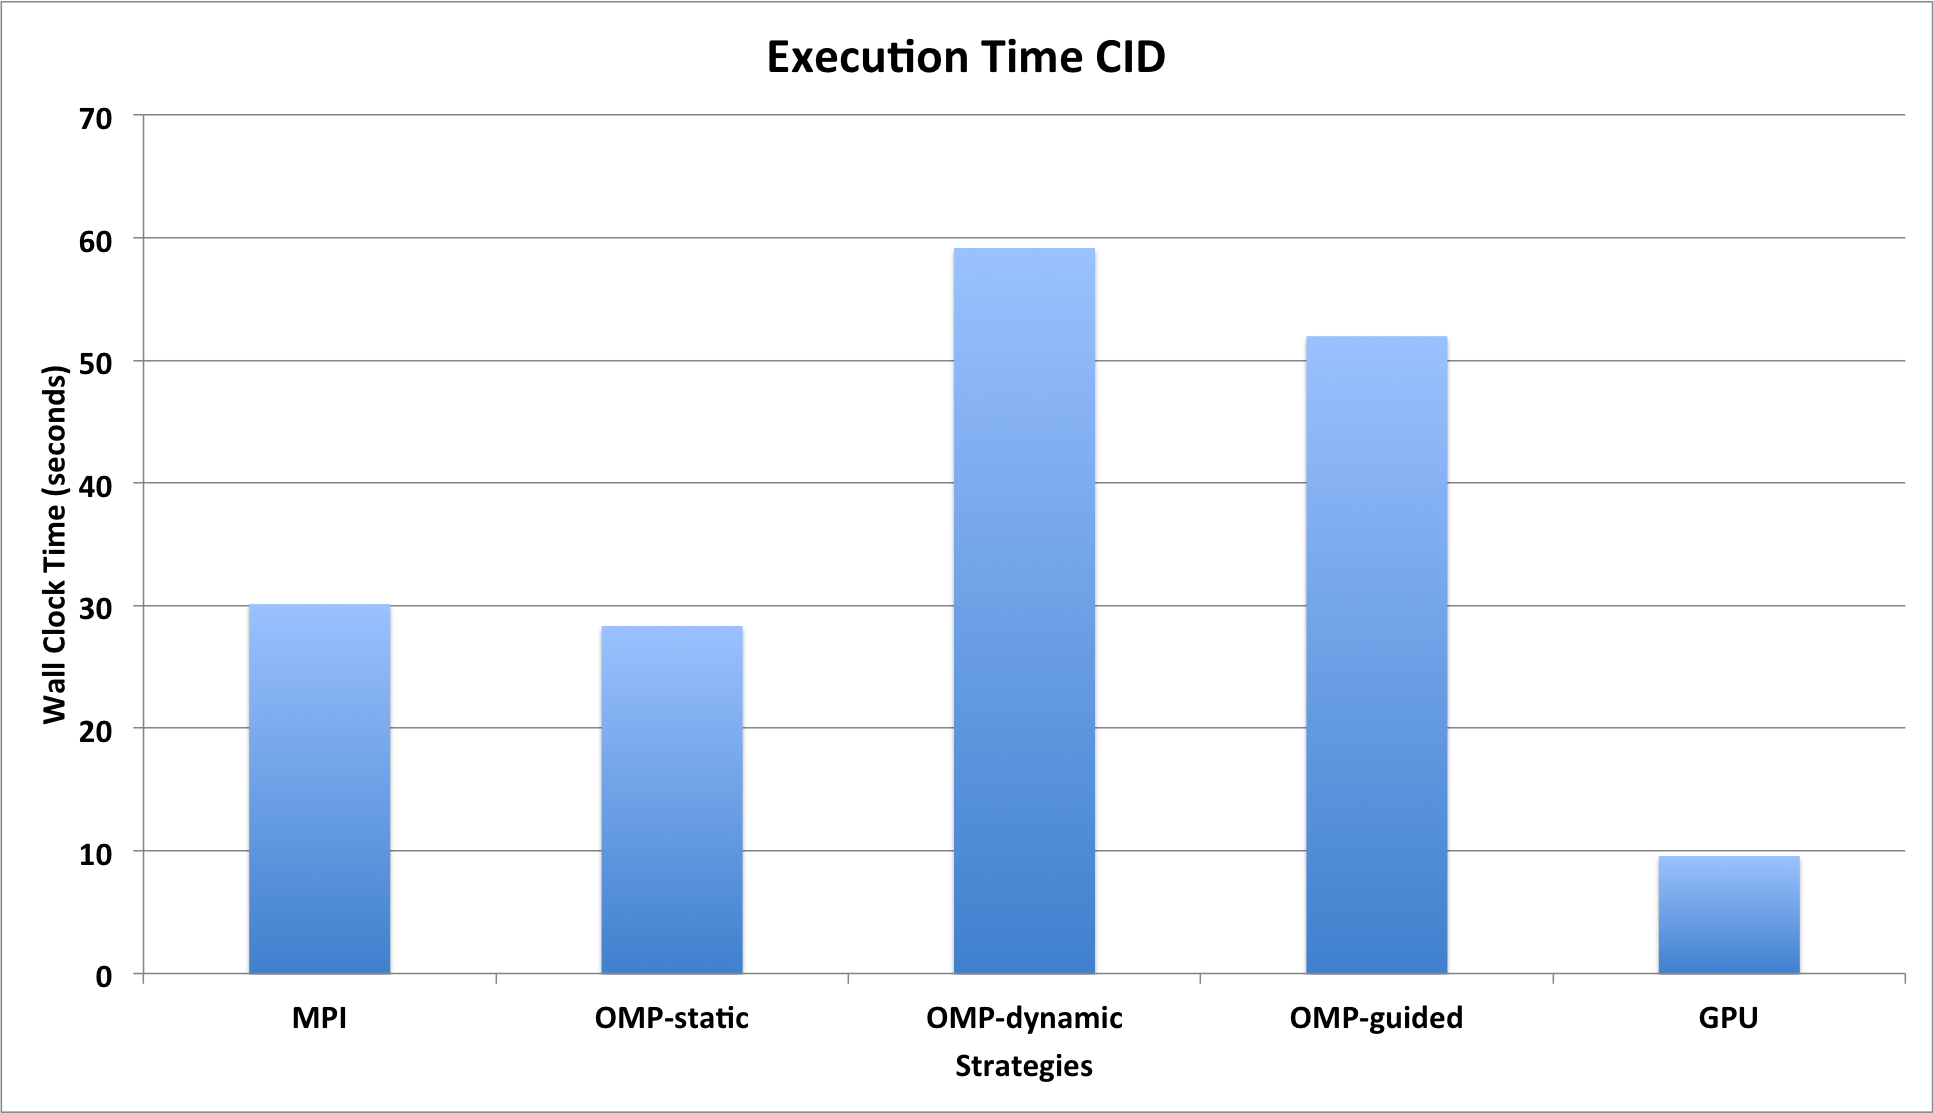
\includegraphics[scale=0.18]{./plots/CIDGPUresults} 
\end{center} 
\end{frame}}  

\comments{
\begin{frame} 
\frametitle{Timing the Functions}  

Used pgcc compiler
\end{frame}
}

\begin{frame}[label=strnrt]
\frametitle{PlasComCM Results/Projections for StrnRt} 

\begin{itemize} 
\tiny \item \tiny Ran PlasComCM code with 2D axi-symmetric problem as input on one node of the xpacc
cluster. 
\item \tiny One MPI process / OpenMP thread per core used for CPU
version. 
\item \tiny Timing done for the StrnRt function only. 
\end{itemize} 

\begin{center} 
% 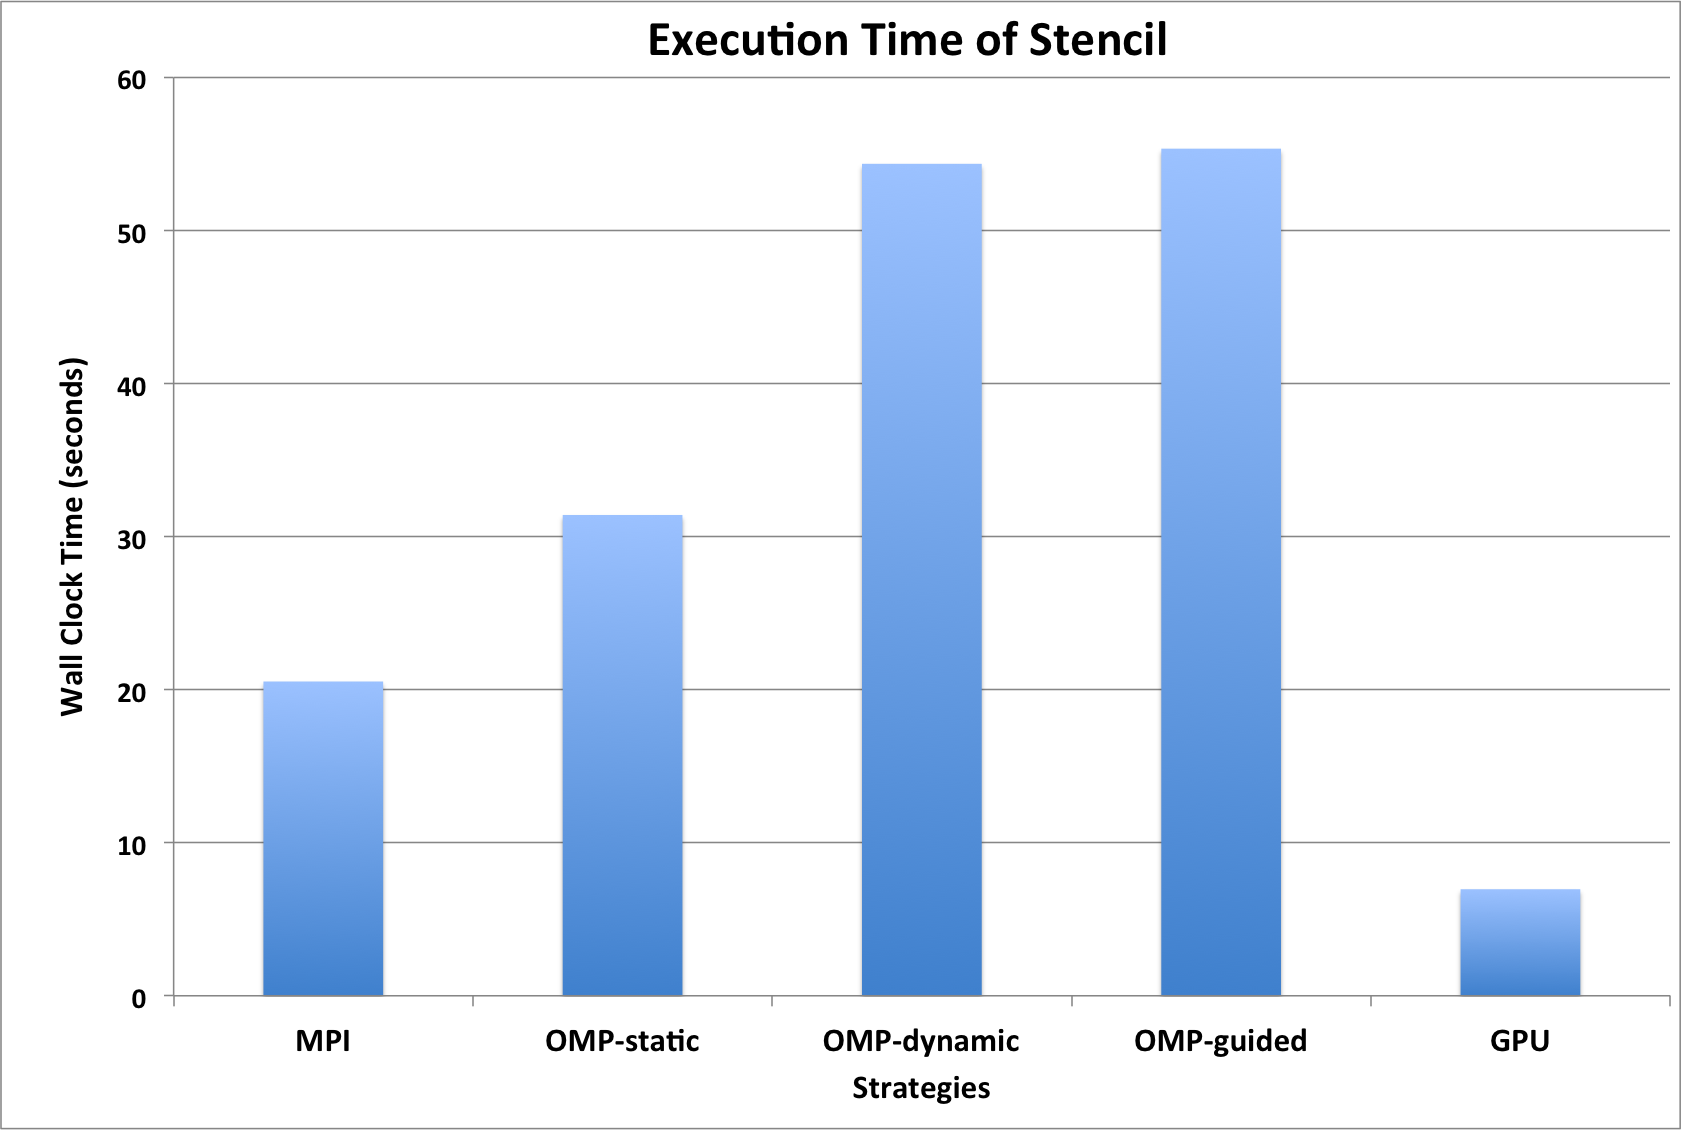
\includegraphics[scale=0.18]{./plots/stencilGPUresults} \hspace*{0.2in} 
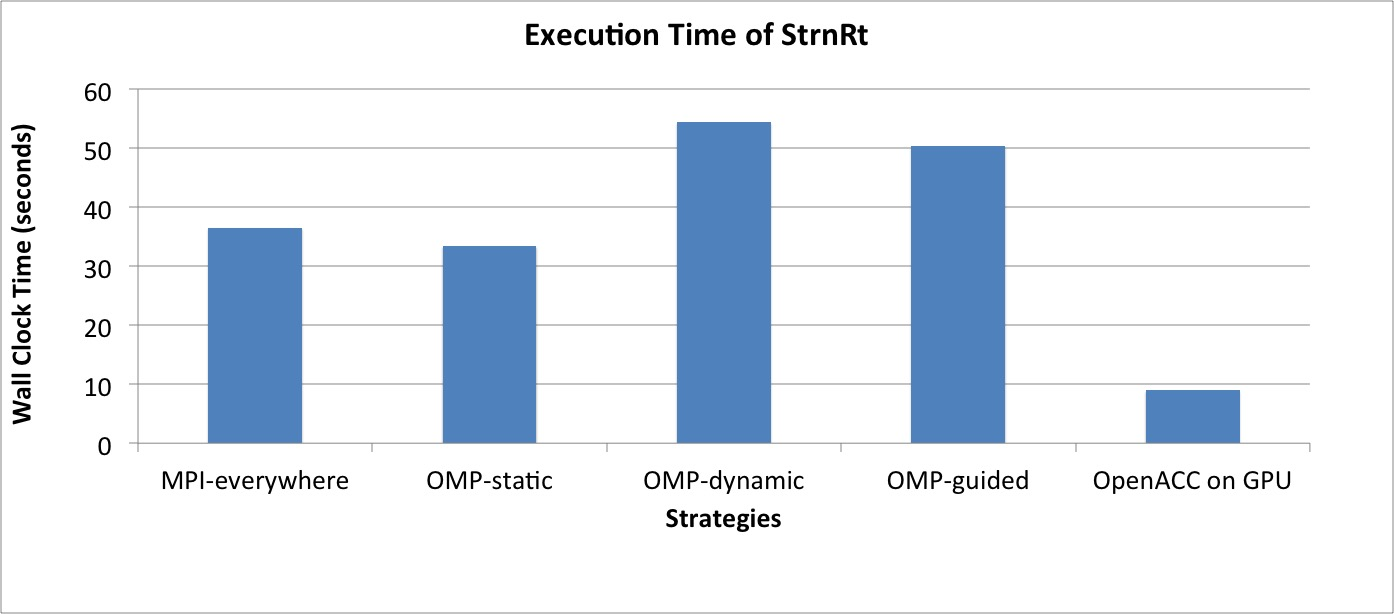
\includegraphics[scale=0.22]{./plots/StrnRtGPUresults} 
\end{center}

\begin{enumerate} 
\tiny \item \tiny OpenMP version with static scheduling run on CPU degrades performance. 
\item \tiny MPI version run on CPU gets 3x performance improvement
  over OpenACC version on GPU. 
\end{enumerate} 
\end{frame} 
\comments{
\begin{frame} 
  \frametitle{How it Fits in the Bigger Picture}
\end{frame} 
}

\begin{frame}[label=impqual]
\frametitle{Questions that follow: Implementation Quality} 
\begin{columns} 
\column{0.5\columnwidth}
\underline{\textbf{CPU }}
\begin{itemize} 
\small \item \small memory bandwidth limitation $\rightarrow$ measure
off-chip cache misses.
\item \small performance variations $\rightarrow$ calculate idle time 
\item \small Others?
\end{itemize}

\column{0.5\columnwidth}
\underline{\textbf{GPU } } 
\begin{itemize} 
\small \item \small Vectorization of code $\rightarrow$ compiler's vectorization report.
\item \small Efficient of use of GPU cores i.e.,  $\rightarrow$ calculate floating point intensity 
\item \small Others? 
\end{itemize} 
\end{columns} 
\end{frame} 

\begin{frame}[label=relatedWork]
\frametitle{Related Work} 
\begin{itemize} 
%\small \item \small PlasComCM paper

\small \item \small Exploring Programming Multi-GPUs Using OpenMP and OpenACC-Based Hybrid Model. Rengan Xu, Sunita Chandrasekaran, Barbara Chapman. 
\item \small Hyesoon Kim, Richard Vuduc, Sara Baghsorkhi, Jee Choi,
  and Wen mei Hwu. Performance analysis and tuning for general purpose graphics processing units (GPGPU). Synthesis Lectures on Computer Architecture. Morgan \& Claypool Publishers, San Rafael, CA, USA, November 2012.
%\item \small GPU paper
%Work-stealing/Cilk: Leiserson and group at MIT 
%Schedule all events together to make only
%  some timesteps be impacted by noise, but can't co-schedule all events.
\end{itemize}
\end{frame} 

%\small \item \small Original MPI code run on CPU with 16 cores: 34.45 ms
%\item \small Transformed OpenACC code run on GPU: 8.34 ms 

\begin{frame} 
\frametitle{Conclusions}
\begin{enumerate} 
  \small \item \small Need low-overhead scheduling strategies for
      improving performance of scientific applications.
    \item \small Many different factors when running an application on a particular architecture. These require multiple low-overhead scheduling strategies to be used at once.
%    \item \small Results show that composition is additive in
%      performance.
   \item \small Future work: (a) Integration with OpenMP or other
      shared memory model; (b) composition with other scheduling
      strategies (which includes generalized methodology for composition for future scheduling strategies). 
%\small \item \small Using GPU can be beneficial for PlasCom over MPI version, if not for
%  current machines, then for future machines. 
\item \small Using OpenACC-ized version of PlasComCM on GPU could be
beneficial over MPI version of PlasComCM on CPU. 
\small \item \small Using OpenACC-ized version of PlasComCM on GPU is
also likely beneficial over OpenMP-ized version of PlasComCM on CPU. 
\item \small Current results will be extended upon to show feasibility. 
\end{enumerate} 
\end{frame} 


\begin{frame}[label=ack] 
  \frametitle{Acknowledgements}
  \begin{itemize}
  \item John Larson - performance models and implementation discussion
%  \item Simon Garcia - discussion of OpenCL code
  \item Jon Freund - Guidance for overall project
  \item Luke Olson - Discussion of input problem sizes
  \item Micheal Klemm - Discussion of OpenACC
  \item Dan Bodony -  Ongoing discussion of PlasComCM data partitioning
%  \item Todd Gamblin: Software
%    \item Franck Cappello: Noise modeling based on fault-tolerance models  
%    \item Torsten Hoefler: amplification and slack description 
%    \item Laura Grigori: CALU scheduling 
%    \item Micheal T. Heath: Suggestions on theoretical analysis and
%      formalization of performance models. 
  \end{itemize}
\end{frame} 

\comments{
\begin{frame}[plain,c]
  \begin{center}
      Appendix
  \end{center}
\end{frame} 
}

\comments{
\begin{frame}[label=mitigationWithinNode]
\frametitle{Within-node Persistent Load Imbalance and Mitigation}
\begin{figure}[ht!]
\label{fig:AppPersistentImbPic}
\subfloat[\tiny Application
  imbalances.]{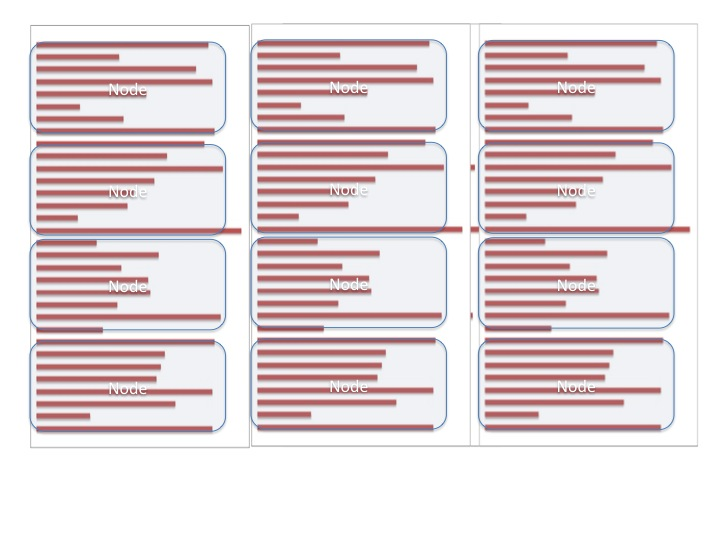
\includegraphics[height=1.3in]{./pictures/PersistentImb2}}\label{fig:AmplificationPic3}\hspace*{0.25in}\subfloat[\label{fig:AmplificationPic3}\tiny
  Mitigated by within-node
  re-distribution.]{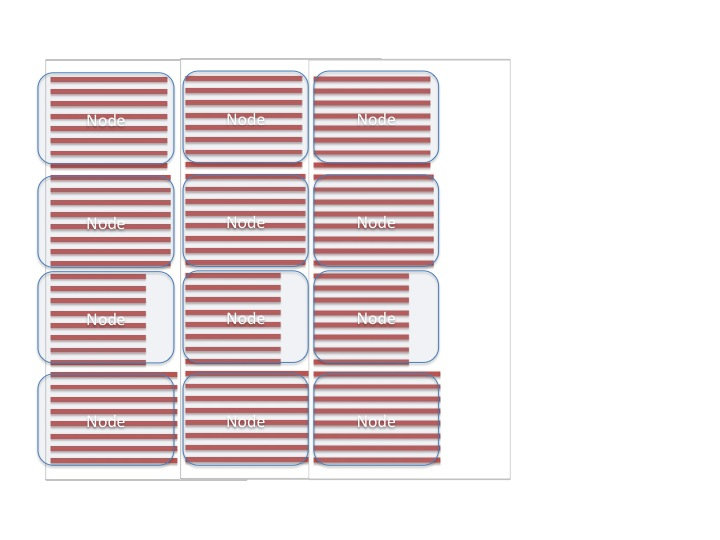
\includegraphics[height=1.3in]{./pictures/PersistentOptimized}}
%\caption{\label{fig:AppPersistentImbPic} Application-induced load
%imbalances.}                                      
\end{figure}
{\small Indent due to not doing across-node balancing, but still much better than before.}
\end{frame}
}

\comments{}